\documentclass[UTF8,titlepage]{ctexart}
\usepackage{amsmath,amssymb,amsthm,amsfonts,amscd}
\usepackage{fontspec}
\setmainfont{Times New Roman}
\usepackage{graphicx}
\usepackage{titlesec}
\usepackage{makecell}
\usepackage{longtable}
\usepackage{xcolor}
\usepackage{tcolorbox}
\usepackage{soul}
\usepackage{adjustbox}
\usepackage{tcolorbox}
\usepackage{enumerate}
\usepackage{pdfpages}
\usepackage{float}
\usepackage{colortbl}
\usepackage{tabularx}
\usepackage{multirow}
\usepackage{pgfplots}
\numberwithin{figure}{section}
\usepackage[left=1.25in,right=1.25in,%
top=1in,bottom=1in]{geometry}
\usepackage{color}
\titleformat{\section}
  {\raggedright\LARGE\bfseries}{\thesection}{1em}{}
\begin{document}
\section{课题一的程序流程图}
\begin{figure}[H]
\centering
 \resizebox{0.5\textwidth}{!}{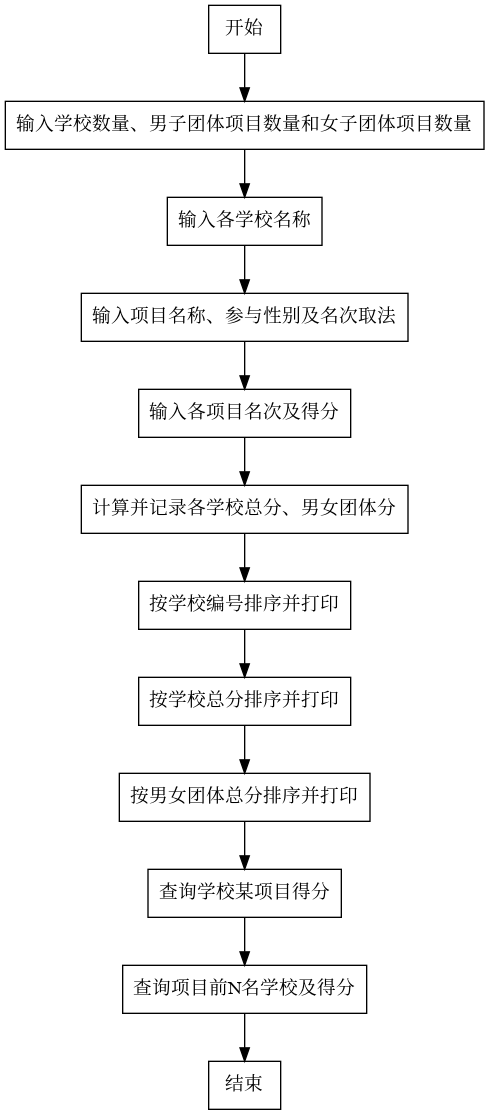
\includegraphics{./fig/program_flowchart.png}}
 \caption{课题一的程序流程图}
 \label{}
\end{figure}
\clearpage
\section{课题二的数据结构}
本课题中用到了以下数据结构:
本代码中使用了以下几种数据结构:
\begin{enumerate}
    \item \textbf{数组(顺序结构)}: 代码中的Car c[10];就是一个数组的例子。数组是一种最基本的数据结构,其元素在内存中是连续的,每个元素可以通过索引直接访问。这是顺序结构的典型特点。数组的优点是访问速度快,但其大小需要在创建时定义,因此在大小变动较大的情况下可能会浪费空间或导致溢出。
    \item \textbf{栈(顺序结构)}: 本代码中的Stack数据结构就是一个栈的实现,采用了顺序结构。栈是一种特殊的线性表,只允许在一端(称为栈顶)进行插入和删除操作。它遵循后进先出(LIFO)的原则。栈可以方便地存储和获取数据,但由于其顺序结构的特性,会存在空间浪费的问题。
    \item \textbf{队列(链式结构)}: 本代码中的LinkQueue数据结构就是一个队列的实现,它采用了链式结构。队列是一种特殊的线性表,只允许在一端(称为队尾)进行插入操作,而在另一端(称为队头)进行删除操作,遵循先进先出(FIFO)的原则。链式结构的队列可以根据需要动态分配和释放存储空间,因此不会浪费空间,但访问元素通常需要从队头开始,因此访问速度较慢。
\end{enumerate}

除此之外,本学习还学习了以下数据结构:
\begin{enumerate}
    \item \textbf{链表}:链表是一种常见的线性数据结构,其中每个元素都包含一个指向下一个元素的指针。链表可以动态地添加和删除元素,所需的空间可以在运行时分配。根据链表的特性,它们可以进一步分类为单链表、双链表、循环链表等。

    \item \textbf{树}:树是一种非线性数据结构,用于表示具有层次关系的数据。树的每个元素(称为节点)都有零个或多个子节点,除了根节点外,每个节点都有一个父节点。常见的树结构包括二叉树、二叉搜索树、堆、平衡二叉树(如 AVL 树)和 B 树等。
    
    \item \textbf{图}:图是一种非线性数据结构,用于表示元素间多对多的关系。图由节点(顶点)和边组成,边可以有或没有方向,可以有或没有权重。常见的图类型包括无向图、有向图、无向加权图、有向加权图等。
    
    \item \textbf{哈希表}:哈希表是一种用于快速查找和插入的数据结构。它通过一个哈希函数将元素映射到一个大的数组中,通过哈希函数和数组索引可以快速找到和存储元素。
\end{enumerate}
\clearpage
\section{课题三的时间复杂度}
\subsection{对于Q-learning}

\begin{enumerate}
\item isValidMove 函数的时间复杂度为 $O(1)$。
\item chooseAction 函数的时间复杂度为 $O(1)$。
\item updateQValues 函数的时间复杂度为 $O(a)$。其中 $a$ 是行动的种类数(在这里是 8)。在函数中的循环遍历了所有可能的动作,循环次数是一个常数。
\item qLearning 函数的时间复杂度为 $O(e \cdot s \cdot a)$。层循环执行总的训练轮数 $e$ 次,内层循环执行每轮训练的最大步数 $s$ 次,而内层循环中的操作的时间复杂度是 $O(a)$。
\item 总时间复杂度为 $O(e \cdot s \cdot a)$。
\end{enumerate}

\subsection{对于DFS}

\begin{enumerate}
\item isValidMove 函数的时间复杂度为 $O(1)$。
\item dfs 函数的时间复杂度为 $O(n \cdot m)$。在最坏情况下,DFS 遍历了整个迷宫的所有单元格,因此时间复杂度与迷宫的行数和列数成正比。
\item solveMaze 函数的时间复杂度为 $O(n \cdot m)$。与 dfs 函数的时间复杂度相同。
\item 总时间复杂度为 $O(n \cdot m)$。
\end{enumerate}
其中
n 表示迷宫的行数(numRows)。

m 表示迷宫的列数(numCols)。

\end{document}